\chapter{Attaques et défenses}


\section{Attaque}
\label{sec:att-def:attaque}


\subsection{Description de l'arme}


Avant d'entrer dans le détail des attaques nous aurons besoin de différentes notions concernant les armes.
La notion de vrai et faux tranchants permet de distinguer avec quelle partie de l'arme nous attaquons : la dénomination provient des épées (principalement les sabres) qui n'étaient affûtés que d'un seul côté (le vrai tranchant).
L'arme est divisée en longueur en trois parties : le fort (proche de la garde), le faible (bout de l'arme) et le milieu (entre les deux).
Parfois le milieu est omis et l'arme est simplement divisée en deux.
Le faible porte ce nom car il est très facile de travailler l'arme et de la dévier en appuyant ou en percutant sur cette partie.
D'un autre côté elle est aussi beaucoup plus mobile et il peut être facile d'esquiver une tentative de percussion.


\begin{definition}[Vrai et faux tranchant]
\label{att:def:tranchant}
\index{tranchant}

Le vrai tranchant désigne la partie de l'arme qui se trouve face à l'adversaire quand l'arme est tenue normalement (garde à droite pour un droitier).
À l'inverse le faux tranchant désigne la partie à l'arrière.
\end{definition}


\begin{definition}[Fort, faible et milieu]
\label{att:def:fort-faible}
\index{arme!fort}
\index{arme!faible}

Le fort correspond au premier tiers de l'arme après la garde, le milieu au second tiers et le faible au dernier tiers (figure~\ref{att:fig:arme-fort-faible}).
\end{definition}


\begin{figure}[ht]
	\centering
	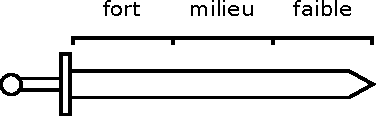
\includegraphics[scale=1.2]{structure/arme_fort_faible.pdf}
	\caption{Fort, milieu et faible sur une arme.}
	\label{att:fig:arme-fort-faible}
\end{figure}


\subsection{Concepts généraux}
\label{sec:att-def:attaque:concepts}


\begin{definition}[Attaques simple et composée]
\index{attaque}

\noindent
On peut distinguer les attaques simples des attaques composées :
\begin{itemize}
	\item une \emph{attaque simple} consiste en un coup isolé ;
	\item une \emph{attaque composée} (ou technique) est une séquence d'actions, chacune ayant pour objectif de préparer la suivante.
\end{itemize}
\end{definition}


Le principal intérêt d'une attaque simple est de tester l'adversaire (type de réaction, temps de réponse…) ou de le faire réagir (forcer un changement de garde…).
Des attaques simples peuvent être enchainées sans pour autant former une attaque composée : par exemple on peut induire un schéma en attaquant alternativement à gauche et à droite avec des coups de taille, pour ensuite le briser et surprendre l'adversaire.

Une attaque composée se distingue d'une attaque simple principalement par l'intention : chaque composante de l'attaque est différente et permet de préparer le terrain.
L'exemple le plus simple d'une attaque composée est une feinte sur une cible suivie d'une attaque sur une autre ouverture : si la feinte est crédible l'adversaire cherchera à se défendre contre la première attaque ce qui ouvre une autre ligne, et du fait que l'attaquant ne porte pas son coup jusqu'au bout il dispose d'une avance (en plus de l'effet de surprise).
L'idée générale est de placer l'opposant dans une situation qui le forcera à réagir d'une manière que nous pouvons exploiter : en effet face à une situation donnée il existe un certain nombre de réactions possibles (conditionnées en partie par l'arme, le style et l'expérience).
Cela explique l'intérêt d'apprendre des techniques : on dispose alors d'un vaste répertoire de pièces que nous pouvons exécuter afin de prendre l'avantage, que nous ayons pris l'initiative ou non à l'origine.
Toutefois il faut être prêt à changer son plan si l'adversaire ne réagit pas comme prévu ou si l'on perçoit une opportunité : ainsi si l'on veut exécuter une feinte mais que l'adversaire ne se protège pas alors il faut porter la frappe jusqu'au bout.
Afin d'être prêt à changer ses plans, et en particulier à transformer une feinte en une vraie attaque, demande à ce que l'on soit souple dans les mouvements.

% TODO: changer de section ?

Une attaque s'accompagne d'un mouvement de jambes qui permet de donner plus de force au mouvement et de sortir de l'axe (définition~\ref{dep:def:sortie-axe}).
En effet si l'attaque se fait en avançant droit devant il y a le risque d'un coup double si l'adversaire fait de même.


\begin{coup}[Attaque normale]
\label{att:coup:attaque-normale}
\index{coup}
\index{attaque|see{coup}}

Partant d'une garde avec le pied droit (resp.\ gauche) en arrière, l'attaquant porte un coup depuis son côté droit (resp.\ gauche) en avançant le pied droit (resp.\ gauche).
L'attaque s'accompagne d'un changement de garde.
\end{coup}

Le fait que le pied et l'attaque ait lieu du même côté s'expliquer par le fait que le coup est plus puissant de cette manière : dans le cas contraire, appeler contre-pied, le mouvement n'est pas naturel pour le corps (voir le commentaire dans Ringeck~\cite[p.~7]{Ringeck:Farrell:2014:CodexRingeck}).
Toutefois il peut arriver que l'on souhaite attaquer du côté où se trouve le pied avant (par exemple redoubler une attaque) : dans ce cas on effectuera quand même un déplacement des pieds accompagné d'une sortie d'axe.
À noter aussi que pour certaines armes, comme l'épée longue~\cite[p.~10]{Ringeck:Farrell:2014:CodexRingeck}, il est conseillé d'attaquer en premier du côté dominant car on pourra y mettre plus de force : ainsi un droitier devrait commencer par attaquer à droite, et inversement pour un gaucher.


\begin{coup}[Attaque du même côté]
\label{att:coup:attaque-même-côté}

Partant d'une garde avec le pied droit (resp.\ gauche) en avant, l'attaquant porte un coup depuis son côté droit (resp.\ gauche) en avançant le pied droit (resp.\ gauche).
Dans ce cas-là il n'y a pas de changement de garde.
\end{coup}


En changeant de garde lors de l'attaque~\ref{att:coup:attaque-normale} on peut bouger un ou deux pieds : soit le pied arrière passe à l'avant simplement (et le pied qui était à l'avant pivote juste), soit ce mouvement est suivi d'une rotation en déplaçant le pied arrière, auquel cas la frappe se fait sur ce deuxième mouvement.

\index{prise}
Lorsqu'une attaque est exécutée il faut veiller à ne pas casser le poignet : l'arme et le bras doivent former ensemble un angle droit (figure~\ref{attdef:fig:poignet-cassé}).
On pourrait avoir l'impression que casser le poignet permet de gagner en allonge, mais en réalité cela cause plusieurs problèmes importants :
\begin{itemize}
	\item lorsque le poignet est cassé nous ne pouvons pas mettre de la force dans l'arme et l'adverse peut la contrôler plus facilement ;
	
	\item cela augmente les risques de blessure, à court et long termes ;
	
	\item la position est moins hermétique et l'adverse dispose de plus de cibles.
\end{itemize}
En effet placer le poignet en extension n'est pas une position naturelle (a fortiori en tenant une arme d'un kilogramme), et on sent très vite que l'on ne peut pas garder cette position longtemps.
Ainsi que nous l'avons vu dans les chapitres précédents toute position inconfortable indique qu'il faut changer quelque chose.


\begin{figure}[ht]
	\centering
	\subfloat[Prise correcte.]{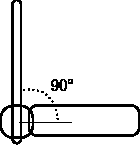
\includegraphics[scale=1]{structure/prise_poignet_correct.pdf}}
	\hspace{3cm}
	\subfloat[Poignet cassé.]{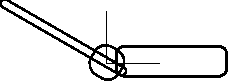
\includegraphics[scale=1]{structure/prise_poignet_casse.pdf}}
	\caption{Comparaison entre une prise correcte et une prise avec le poignet cassé.}
	\label{attdef:fig:poignet-cassé}
\end{figure}

% cf escrime japonaise

L'attaque à contre-pied va à l'opposé de l'attaque normale telle qu'elle a été décrite plus haut.
Elle permet de gagner en distance et de surprendre l'adversaire.
Le gain de distance par rapport à la position normale est due à la position des épaules.

\begin{coup}[Attaque à contre-pied]
\label{struct:coup:contre-pied}
\index{coup!en contre-pied}
\index{contre-pied|see{coup}}
\index{coup!croisé|see{contre-pied}}

Une attaque à contre-pied (ou coup croisé) consiste à avancer le pied du côté opposé à celui où l'on attaque.
\end{coup}


Il existe trois types de coups : la taille, l'estoc et l'entaille -- celle-ci n'étant possible qu'avec des armes tranchantes.
Chacune de ses frappes est plus ou moins adaptée selon l'arme utilisée, mais aussi selon la situation.


\begin{coup}[Taille]
\index{coup!taille}
\index{coup!haw|see{coup taille}}
\index{haw|see{coup taille}}

La taille (\emph{haw}, littéralement frappe) consiste à frapper avec le bord de l'arme (le tranchant pour une épée).
\end{coup}


\begin{coup}[Estoc]
\index{coup!estoc}
\index{coup!stich|see{coup estoc}}
\index{stich|see{coup estoc}}

L'estoc (\emph{stich}) consiste à frapper avec la pointe de l'arme (dans un mouvement longitudinal).
\end{coup}


\begin{coup}[Entaille]
\index{coup!entaille}
\index{coup!schnitt|see{coup entaille}}
\index{schnitt|see{coup entaille}}

L'entaille (\emph{schnitt}) consiste à faire glisser le tranchant de l'arme le long de la cible.
\end{coup}


Une technique typiquement inclue une combinaison de ces différentes frappes, et certaines s'enchaînent naturellement.
Par exemple après un coup de taille on peut enchaîner avec :
\begin{itemize}
	\item un estoc si l'on a pris le centre et que notre pointe se trouve face à l'adversaire ;
	\item une entaille si la frappe est arrive contre le corps de l'adversaire.
	% typique Katori
\end{itemize}


Finalement les coups de tailles peuvent être portés dans trois directions différentes : descendant (coup supérieur, ou d'en haut), montant (coup inférieur, ou d'en bas) et latéral.
Dans le premier cas l'attaque part typiquement d'une garde haute et termine dans une garde basse, et inversement pour le coup du bas.


\begin{coup}[Coup descendant (supérieur)]
\label{att:coup:descendant}
\index{coup!descendant}

Un coup descendant consiste à frapper du haut vers le bas, en général selon une trajectoire diagonale.
\end{coup}


\begin{coup}[Coup montant (inférieur)]
\label{att:coup:montant}
\index{coup!montant}

Un coup descendant consiste à frapper du bas vers le haut, en général selon une trajectoire diagonale.
\end{coup}


\begin{coup}[Coup latéral (intermédiaire)]
\label{att:coup:latéral}
\index{coup!latéral}

Un coup latéral est un coup horizontal, la trajectoire de la lame étant parallèle au sol.
\end{coup}


Lorsque l'on s'entraîne avec une nouvelle arme il faut s'habituer aux différentes frappes possibles, apprendre à reconnaître lesquelles sont les plus naturelles.


\begin{exercice}[Mouvements dans le vide]
Effectuer des attaques simples dans le vide, puis des enchaînements.

Cet exercice devrait être un des premiers à effectuer avec toute nouvelle arme afin de s'habituer à son poids, à sa taille, aux mouvements possibles avec le corps, etc.
\end{exercice}


\index{appel}
Un des risques lors des attaques est de donner un signal à l'adversaire qui lui permet d'anticiper notre attaque (on parle d'appel).
Cela revient à dire : « attention je vais t'attaquer depuis la droite avec un coup de taille ».
Il faut donc s'entraîner à diminuer autant que possible les mouvements parasites qui précèdent la frappe.
Un appel typique consiste à ramener l'arme légèrement en arrière avant de frapper : cela vient de la croyance que reculer l'arme et lui faire parcourir plus de distance permet de frapper plus fort, alors qu'en réalité le mouvement des hanches est suffisant.
Un autre appel consiste à élever légèrement les épaules, ou même le corps dans son ensemble.

Un autre risque lors de l'attaque est de ne pas se protéger le corps.
Typiquement cela arrive quand on arme le coup en arrière et que l'on commence à avancer : l'arme se trouve derrière soi tandis que le corps commence à se rapprocher, et un adversaire peut facilement attaquer à ce moment.
Il faut donc toujours garder à l'esprit que l'attaque doit être sûre et ne laisse aucune possibilité à l'adversaire de s'insérer entre l'arme et le corps.
Tout attaque doit commencer par gêner l'adversaire, soit en le forçant à réagir, soit à défaut en plaçant notre arme entre lui et nous.
% cf les exercices de kung-fu de Thomas

Lorsque l'on frappe il faut penser à être (relativement) détendu.
En effet si l'on a tendance à crisper le haut du corps (et en particulier les épaules) alors le reste ne peut pas jouer un rôle correct (en particulier les hanches).
Vu de l'extérieur ce genre de mouvements apparaît artificiel ; et dans la pratique il est souvent peu efficace (ou du moins beaucoup qu'il ne le serait avec une mécanique correcte).
Il faut donc apprendre à donner de la force et à contrôler sa frappe mais sans se bloquer.


\begin{exercice}
\label{att:ex:marche-poing-détendu}

\A exécute une marche avant en donnant un coup de poing, puis il revient détendu en garde pour mieux absorber l'impact (donc le bras ne reste pas tendu).
\end{exercice}



\subsection{Cibles}


Les cibles précises dépendent de l'arme considérée mais il existe certaines idées générales.
Une cible intéressante est ouverte : cela signifie que l'adversaire ne la protège pas et qu'il va lui falloir un temps de réaction avant de pouvoir le faire.
L'idée générale est donc de créer une ouverture, en conduisant l'adversaire à ne pas protéger une partie de son corps que l'on peut ensuite attaquer.

Rappelons que pour tous les exercices de frappe (et surtout sur une cible immobile) il est vital de s'arrêter \emph{avant} le contact (environ \SI{10}{cm}), et en particulier pour les estocs ou les coups à la tête.
Savoir s'arrêter à temps fait aussi partie de l'entraînement et démontre que l'on sait contrôler nos coups, que ce soit en vitesse ou en précision.
Quelqu'un qui ne sait pas contrôler ses frappes et qui blesse ses partenaires n'a aucune excuse et n'a pas compris le principe de l'escrime.
Toutefois il est peut être utile d'aller jusqu'au contact pour vérifier quelque chose ou si l'exercice le requiert, mais uniquement \emph{après accord} du partenaire (et même dans ce cas-là le coup ne doit pas conduire à une blessure).


\begin{definition}[Ouverture]
\index{ouverture}

Une ouverture correspond à une cible qui n'est pas protégée (au moment où l'attaque est initiée).
\end{definition}


On distingue entre les cibles hautes et basses selon leur position : les premières regroupent la tête, le torse et les bras, les secondes les jambes et le bas du torse.


\begin{definition}[Cibles basse et haute]
\index{cible!basse}
\index{cible!haute}

Une cible est dite haute/basse si elle se trouve au-dessus/en-dessous de la ceinture (nombril).
\end{definition}


\begin{exercice}
\begin{enumerate}
	\item \D place une cible dans laquelle \A donne un coup de poing.
	
	\item \D recule et change la position de la cible, puis \A attaque encore (à répéter).
\end{enumerate}
\end{exercice}


\begin{exercice}
\begin{enumerate}
	\item \D place une cible basse dans laquelle \A donne un coup de pied.
	
	\item \D déplace la cible sur le côté et \A se déplace et donne deux coups de poing.
\end{enumerate}
\end{exercice}


Il est évident que la tête est une cible importante, mais il peut être beaucoup plus intéressant de viser le torse -- plus grande superficie -- ou les membres (appelés aussi avancées) -- plus faciles à atteindre.
Pour cette raison il est important de toujours s'assurer que l'avant-bras ne peut pas être facilement atteint par l'adversaire à chaque fois que l'on attaque (en particulier si l'on dispose d'un bouclier celui-ci doit couvrir le bras).
En effet il suffit d'une blessure suffisamment importante au bras d'arme pour empêcher l'adversaire de continuer le combat : dans ce cas il n'y a aucune raison logique de vouloir viser absolument la tête ou le torse.
Comme nous en avons déjà parlé dans l'introduction le point clé est de mettre fin au combat le plus vite possible -- en survivant.
Attaquer le bras est particulièrement intéressant car si l'on se trouve juste à portée pour frapper le bras cela signifie que nous sommes hors distance par rapport à l'arme de l'opposant (si les armes sont similaires).


\begin{coup}[Attaques aux avancées]
\index{attaque!aux avancées}

Une attaque aux avancées consiste à attaquer le bras (ou parfois la jambe) de l'adversaire, en général suite à une attaque de celui-ci.

\end{coup}


% TODO: améliorer
\begin{exercice}[Attaques aux avancées]

\begin{enumerate}
	\item \A porte une attaque simple sur \D et arrête le coup avant la touche.
	
	\item \D vérifie s'il peut facilement blesser \A au bras.
\end{enumerate}

L'exercice peut être modifié, par exemple en permettant à \D de se protéger ou d'esquiver (avec un pas), ou bien en n'autorisant \D à toucher \A que s'il se trouve en sécurité.
\end{exercice}


\begin{exercice}
\A et \D n'ont aucune protection.

\A porte une attaque et touche \D (juste un contact léger), à ce moment \D attaque \A (sans s'être protégé), et ainsi de suite.

L'idée de l'exercice est de perdre la peur d'être touché par l'arme de son équipier tout en apprenant à gérer sa force et la distance.
\end{exercice}


\index{coup!jambe}
Il faut noter que les attaques à la jambe peuvent être dangereuses car l'on se trouve dans une position où la tête est à portée.
L'adversaire peut facilement retirer la jambe prise pour cible tout en attaquant à la tête.
Il faut donc réserver ce genre d'attaques dans les cas où la tête peut être protégée efficacement (par exemple avec un bouclier) ou si l'adversaire peut être suffisamment pris au dépourvu.

La logique même indique qu'il est plus efficace d'attaquer aux ouvertures plutôt que là où l'adversaire se défend.
Ainsi si l'arme se trouve d'un côté on attaquera prioritairement de l'autre : cela est d'autant plus naturel lorsque les deux adversaires sont droitiers et adoptent une garde à droite, auquel cas le côté gauche est ouvert et se trouve en face de l'arme.
Toutefois ce principe ne tient pas toujours car il peut être dangereux d'attaquer de l'autre côté si l'on a déjà attaqué d'un côté (l'exemple de la série des huit coups~\ref{att:coup:série-8}).

En escrime moderne huit cibles sont privilégiées et ont reçu un nom particulier.
Chacune est associée à une garde et porte le nom de cette dernière.
Afin de faciliter les descriptions nous utiliserons souvent ces dénominations qui ont le mérite d'être claires (en particulier pour les gardes que nous verrons plus loin).


\begin{coup}[Escrime moderne]
\label{att:coup:série-8}
\index{coup!escrime moderne}

\noindent
Les huit frappes d'escrime moderne sont :
\begin{enumerate}
	\item prime : attaque basse à droite ;
	\item seconde : attaque basse à gauche ;
	\item tierce : attaque haute à gauche ;
	\item quarte : attaque haute à droite ;
	\item quinte : attaque à la tête ;
	\item sixte : attaque haute à gauche ;
	\item septime : attaque basse à droite ;
	\item octave : attaque basse à gauche.
\end{enumerate}

Les cibles sont résumées sur la figure~\ref{att:fig:série-8}.
\end{coup}


À noter que les trois dernières attaques (resp.\ sixte, septime, octave) ne sont pas différentes des trois premières (resp.\ tierce, prime, seconde) -- par contre les gardes le seront.
Les attaques sont enchaînées en changeant de garde (coup~\ref{att:coup:attaque-normale}), à l'exception de celles sur la seconde et la tierce, qui se font du même côté (coup~\ref{att:coup:attaque-même-côté}).
L'explication du début de l'enchaînement est la suivante : en 1) \A attaque l'ouverture à la gauche de \D qui se trouve en garde à droite, en 2) \A attaque l'ouverture créée à droite, en 3) il est trop dangereux d'aller attaquer de l'autre côté donc \A attaque encore la droite de \D, mais en haut, en 4) \A peut maintenant attaquer l'ouverture à gauche.
Cela explique pourquoi \A attaque deux fois du même côté même si cela peut paraître étrange à première vue.


\begin{figure}[ht]
	\centering
	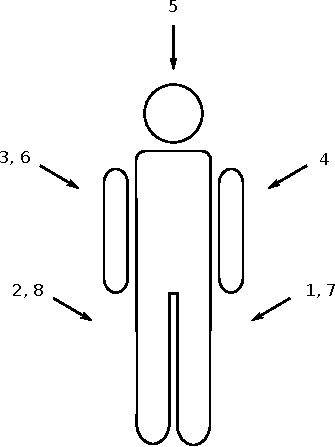
\includegraphics[scale=1]{structure/attaques_set_8.pdf}
	\caption{Frappes en escrime moderne.}
	\label{att:fig:série-8}
\end{figure}


Deux exercices très simples consistent à exécuter dans l'ordre les coups ci-dessus : d'abord les cinq premiers, puis tous les coups.
Cela permet d'apprendre à placer ses frappes et à vérifier la précision tout en s'habituant à l'arme.
Une fois que le mouvement de base est acquis l'exercice peut être modifié afin de travailler d'autres concepts, comme les déplacements.
La cadence peut aussi être accélérée.


\begin{exercice}[Série de cinq]
\index{echauffement@échauffement!exercice}

\obj{Travailler le mouvement de la frappe et la précision.}

\begin{itemize}
	\item \D attend sans bouger pendant que \A exécute les cinq premiers coups~\ref{att:coup:série-8}.
	
	\item Les rôles sont inversés.
\end{itemize}

Quand les mouvements sont acquis \D commence l'enchaînement aussi vite que possible après que \A ait fini.
\end{exercice}


\begin{exercice}[Série de huit]

\obj{Travailler le mouvement de la frappe et la précision.}

\begin{enumerate}
	\item \D attend sans bouger pendant que \A exécute les huit coups~\ref{att:coup:série-8}.
	
	\item Les rôles sont inversés.
\end{enumerate}

Quand les mouvements sont acquis \D commence l'enchaînement aussi vite que possible après que \A ait fini.
Dans ce cas il peut arriver que \A ne parvienne pas à se protéger en prime si \D attaque directement depuis l'octave : il s'agit de tourner le poignet en changeant de garde (en reculant), ce qui permet de placer la pointe vers le ventre de l'adversaire (en tournant encore un peu le poignet on peut avancer et trancher à la place d'estoquer).
\end{exercice}


\begin{exercice}[Série avec garde]

\obj{Travailler les déplacements.}

\D attend en garde sans bouger pendant que \A exécute les cinq premiers ou l'ensemble des huit coups~\ref{att:coup:série-8}, puis les rôles sont inversés.

La garde qui permet de faire travailler au maximum les déplacements est la longue pointe, qui consiste à se tenir en garde avec l'épée droit devant.

\end{exercice}


\begin{exercice}[Série complète]

\obj{Travailler l'ensemble des coups possibles.}

\D attend sans bouger pendant que \A exécute l'ensemble des combinaisons possibles pour les frappes (estocs, tailles montantes/descendantes/horizontales) et les cibles (cibles hautes et basses).
Un récapitulatif est donné dans la figure~\ref{att:fig:série-complète}, avec une suggestion de l'ordre des attaques (mais rien n'empêche de varier pour tester différentes combinaisons).

Par la suite \D peut se mettre en garde pour compliquer l'exercice.
\end{exercice}


\begin{figure}[ht]
	\centering
	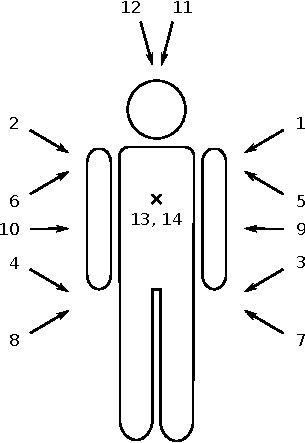
\includegraphics[scale=1]{structure/attaques_set_complet.pdf}
	\caption{Série complète de frappes.
	La croix désigne les deux estocs (un de chaque côté).}
	\label{att:fig:série-complète}
\end{figure}


Une attaque doit viser une cible précise : il n'est pas question d'agiter son épée au hasard en espérant obtenir quelque chose, d'autant plus que cela est dangereux dans le cadre de la pratique sportive.
Ainsi il peut être utile de s'arrêter par moment afin de vérifier que la cible visée a bien été atteinte.
La cible est assimilée à un point dans l'espace : si l'opposant se déplace pour éviter l'attaque il ne faut pas chercher à le suivre (sauf si cela fait partie de la technique), sinon on lui permet de nous amener là où il le décide.
De plus une fois que l'on a atteint la position visée il ne faut pas continuer la coupe jusqu'au bout, car alors on se prête à une riposte : après chaque attaque il faut absolument se retrouver dans une garde qui ne laisse aucune ouverture.
L'adversaire doit être gêné par la position de notre arme après la frappe.
Ainsi que cela a été mentionné plus haut cela implique de ne pas casser le poignet.

D'un point de vue plus pragmatique la précision permet de diminuer le danger pour le partenaire : dans le cadre d'un exercice le coup doit être prévisible car la réaction du partenaire sera accordée sur celui-ci.
En frappant systématiquement au mauvais endroit on augmente les chances de blessure car on risque d'arriver là où le partenaire ne s'y attend pas et n'est pas protégé.

Ainsi le fait de contrôler ses coups (en vitesse et en précision) est tout aussi important que de savoir comment frapper ou comment se défendre.
Sans cela l'escrime ne serait qu'un jeu barbare ou celui qui frappe le plus fort sortirait vainqueur, et auquel cas il n'y a aucun intérêt d'étudier les techniques.


\begin{exercice}[Fermer les yeux]
\obj{Évaluer rapidement une situation et choisir la bonne cible.}

\begin{enumerate}
	\item \A ferme les yeux.
	
	\item \D se déplace et choisit une garde.
	
	\item \D donne un signal (par exemple le nom de \A), \A ouvre les yeux et doit attaquer immédiatement sur une ouverture.
\end{enumerate}

Il est conseillé de porter un masque pour cet exercice.
\end{exercice}


\begin{exercice}

\begin{enumerate}
	\item \A ferme les yeux.
	
	\item \D se déplace et choisit une garde.
	
	\item \D donne un signal (par exemple le nom de \A) et attaque peu après.
	\A ouvre les yeux et doit attaquer immédiatement sur une ouverture.
\end{enumerate}

\end{exercice}



\subsection{Compléments}


Le fait de passer d'une prise en pronation à une prise en supination (ou inversement) tout en gardant la main au même endroit permet de changer la ligne d'attaque.
En particulier cela peut permettre de placer l'épée pour blesser l'adversaire tout en restant soi-même protéger : en effet si l'arme est tournée vers l'extérieur dans la position initiale, le changement pronation/supination permet d'effectuer une rotation de \ang{180} et de passer derrière la garde adverse.


\begin{technique}[Changement de ligne]
\label{struct:tech:changement-ligne}

\A et \D ont les lames en contact, la garde est prise à droite en pronation.
\A tourne sa main en supination afin de passer sa lame derrière celle de \D pour le toucher.

% Source : Romain.
\end{technique}


\section{Défense}


\index{défense}
Nous distinguons deux types de protection : les gardes (passif) et les défenses dynamiques (actif).
Les gardes sont des positions que l'on adopte lors de l'attente et entre chaque attaque.
Les défenses s'exécutent à partir d'une garde et correspondent à une action visant à se protéger d'une attaque.


\subsection{Gardes}


\index{garde|textbf}
\index{défense!garde|see{garde}}
L'objectif d'une garde est multiple.
En premier lieu il s'agit d'une position qui permet de protéger une partie du corps.
Du fait que chaque arme occupe une portion limitée de l'espace cela signifie aussi qu'une autre partie du corps sera plus vulnérable.
\index{invite}
On peut tirer parti de ce fait avant d'encourager l'adversaire à attaquer une cible donnée si l'on connaît le contre adapté -- on parle d'\emph{invite.}
Une garde permet aussi de faciliter certaines attaques : par exemple si on adopte une garde haute à droite il sera plus facile de frapper de taille à droite.

Certaines gardes sont adaptées lorsque sont les combattants se trouvent hors distance (voir définition~\ref{conc:def:distances}) : dans ce cas il s'agit de positions relâchées qui permettent de se reposer et d'observer l'adversaire en attendant le début du combat à proprement parler.
Par exemple on pourra laisser reposer l'épée sur l'épaule.

Un danger est de rester trop longtemps dans une même garde : il devient alors très facile pour l'adversaire de prendre le dessus car il existe plusieurs contres à chaque garde, et plus on restera longtemps dans une garde plus l'adversaire aura de chances d'utiliser l'un d'eux.
Ainsi il faut changer fréquemment de gardes sans passer trop de temps.

Nous allons décrire les huit gardes de l'escrime moderne qui correspondent aux coups \ref{att:coup:série-8}.
Ainsi que nous l'avons expliqué plus haut les gardes d'escrime moderne sont faciles à retenir et à désigner, et elles peuvent être effectuées avec différentes armes ce qui en fait un bon point de départ.
Par la suite nous verrons les gardes historiques adaptées à chaque arme.


\begin{garde}[Escrime moderne]
\label{att:garde:escrime-moderne}
\index{coup!escrime moderne}

\noindent
Les huit frappes d'escrime moderne sont :
\begin{enumerate}
	\item prime : garde basse à gauche en pronation, arme vers le bas ;
	\item seconde : garde basse à droite en pronation, arme vers le bas ;
	\item tierce : garde haute à droite en pronation ;
	\item quarte : garde haute à gauche en pronation ;
	\item quinte : garde au-dessus de la tête, épée horizontale (la main peut être à gauche ou à droite) ;
	\item sixte : garde haute à droite en supination ;
	\item septime : garde basse à droite en supination ;
	\item octave : garde basse à gauche en supination.
\end{enumerate}
\end{garde}


Les trois dernières gardes ne sont pas naturelles avec toutes les armes.
Elles se retrouvent particulièrement à la rapière car elles permettent d'avoir la pointe dirigée vers l'adversaire et d'enchaîner facilement avec un estoc.
Pour les autres armes, et particulièrement celles à deux mains, la prise en supination ne convient que si on exécute une parade de percussion : frapper/balayer la lame ennemie en parant afin de la dégager, en gardant le tranchant à "l'intérieur" (i.e. vers l'ennemi).
Par exemple la sixte avec une épée à deux mains s'effectue en bloquant la poignée dans le creux du coude et contre le bras, et ensuite on peut se projeter en avant pour empaler l'adversaire ou lui trancher la gorge.

Avec une arme à deux mains la prime et la seconde se font en levant les mains au niveau de la tête.
Le passage de tierce en quarte se fait en pivotant le buste : le bras ne bouge que légèrement pour amener la main sur le côté.

Une parade haute se fait de préférence avec les mains du côté de la jambe arrière : de cette manière la pointe est naturellement tournée vers l'adversaire.


\subsection{Défenses actives}


Il existe plusieurs manières de se défendre : la parade franche, l'absorption, la déviation et l'esquive.
Elles se distinguent par l'intensité du contact entre les deux armes.


\begin{definition}[Parade franche]
\index{défense!parade franche}

Une parade franche consiste à se protéger en opposant directement son arme à la frappe adverse.

\end{definition}


\begin{definition}[Absorption]
\index{défense!absorption}

Absorber un coup consiste à accompagner le mouvement afin de réduire l'intensité du coup.

\end{definition}


\begin{definition}[Déviation]
\index{défense!déviation}

Une déviation consiste à changer la trajectoire d'une attaque adverse.

\end{definition}


\begin{definition}[Esquive]
\index{défense!esquive}
% \index{esquive|see{défense}}

L'esquive consiste à éviter une attaque en déplaçant son corps hors de portée.

\end{definition}


Les parades franches peuvent être dangereuses : si l'on se trouve dans une position faible ou si l'adversaire est plus fort il existe un risque que la parade se fasse déborder et que l'on reçoive la frappe de toutes manières.
De plus l'on n'est pas dans une bonne position pour résister après une parade franche.
Pour ces deux raisons il convient d'éviter autant que possible ce genre de parades.


\begin{exercice}

\begin{enumerate}
	\item \A donne un coup circulaire.
	
	\item \D vient stopper le coup en plaçant ses deux avant-bras contre son bras.
	
	\item \D vient toucher l'épaule de \A.
\end{enumerate}
\end{exercice}


\begin{exercice}[Parer en quarte]

\A et \D sont en garde, pied gauche devant.

\begin{enumerate}
	\item \A attaque \D du côté droit (quarte).
	
	\item \D se protège en quarte sans bouger les pieds.
\end{enumerate}

Même s'il ne bouge pas les pieds \D a intérêt à pivoter les hanches afin de parer plus efficacement.

\end{exercice}


La solution la plus simple après la parade franche consiste à absorber la frappe : ainsi une partie de l'énergie est dissipée, et de plus le mouvement associé permet d'accompagner l'arme adverse dans une position qui nous est plus favorable.
L'exemple typique consiste à changer de garde.


\begin{exercice}

\begin{enumerate}
	\item \A donne un coup.
	
	\item \D vient couvrir du bras opposé (avant-bras vertical) en se décalant sur le côté.
	
	\item \D vient toucher l'épaule de \A.
\end{enumerate}

Le fait de venir toucher l'épaule permet d'entraîner le réflexe d'attaquer après s'être protégé ainsi que de solliciter les hanches.
\end{exercice}


\begin{exercice}[Absorber en quarte]

\A et \D sont en garde, pied gauche devant.

\begin{enumerate}
	\item \A attaque \D du côté droit (quarte).
	
	\item \D se protège en quarte en changeant de garde.
\end{enumerate}

En comparant cet exercice au précédent \D doit sentir qu'il peut mieux résister si \A se met à forcer.
\end{exercice}


Une autre possibilité assez instinctive est de dévier l'attaque : dans ce cas nous utilisons notre arme afin de frapper celle de l'adversaire.
L'effet obtenu varie selon l'angle utilisé lors de la percussion : par exemple on pourra dévier la lame sur le côté ou vers le sol.
L'intérêt de la déviation est de permettre de se protéger à moindre effort (comparer à une parade franche) tout en étant dans une excellente position pour attaquer une ouverture.


\begin{exercice}

\begin{enumerate}
	\item \A donne un coup du poing droit.
	
	\item \D dévie l'attaque en se décalant sur le côté.
	
	\item \D vient toucher l'épaule de \A.
\end{enumerate}

Lorsque \D dévie avec la main droite il doit la faire passer par-dessus le bras de \A afin de rabattre son bras sur le côté (les doigts sont alors dirigés vers le sol).

\D doit prendre garde à garder ses doigts serrés (et en particulier le pouce) pour éviter de se blesser.
\end{exercice}

Finalement l'esquive revient à soustraire le corps à l'attaque : l'intérêt étant que l'arme reste disponible pour attaquer immédiatement après.
Toutefois une esquive reste dangereuse et pour cette raison on pourra éventuellement se couvrir avec son arme (c'est-à-dire en la plaçant entre nous et la trajectoire possible de la frappe adverse).


\begin{exercice}
\A touche une épaule, puis l'autre et à la troisième attaque \D se baisse pour esquiver.
\end{exercice}


Une parade franche ou une absorption peuvent être mise à profit pour accrocher l'arme adverse : il s'agit de l'amener dans une position qui nous permet de la contrôler plus facilement (typiquement en coinçant le faible dans les quillons).


\begin{definition}[Accrochage]
\index{défense!accrochage}
\index{accrochage|see{défense}}

Un accrochage revient à bloquer l'arme adverse grâce à notre arme.
\end{definition}


\begin{exercice}
\A porte des coups sur différentes cibles, et à chaque fois \D cherche une esquive, une parade ou une riposte.
\end{exercice}



\section{Changement de garde en deux étapes}


% Thomas (kung fu)
\label{def:texte:garde-kung-fu}
On peut raffiner l'exécution des changements de garde en décomposant clairement les deux processus~\footnotemark{}.
\footnotetext{L'analyse présentée dans cette section est due à Thomas Mainguy.}
En effet un changement de garde implique deux mouvements : un pour chaque pied.
On peut alors tirer parti de cette décomposition en étant conscient de l'existence d'une première étape au lieu de l'exécuter mécaniquement.
Cela permet d'ajouter une action supplémentaire avec l'arme tout en offrant une plus grande flexibilité pour la suite du mouvement.
En particulier le mouvement des hanches lors du premier mouvement amène naturellement l'arme en couverture et permet donc de se protéger, le second mouvement permettant alors de riposter directement.
Le message dont il faut se souvenir est que l'on a le temps d'effectuer ces deux mouvements lors d'un changement de garde.
Il s'agit d'un excellent exemple où l'on voit comment la mécanique du corps (et surtout des hanches) se combine avec le déplacement pour donner lieu à une défense efficace suivie d'une attaque.

\begin{technique}[Changement de garde avant en deux temps]
\label{att:tech:changement-garde-2-temps-avant}

\begin{enumerate}
	\item \A pivote les hanches pour amener le poids sur la jambe avant tout en commençant à avancer la jambe arrière.
	
	\item \A termine le mouvement en pivotant.
\end{enumerate}

\A peut éventuellement ajouter une légère marche ou poussée.

Au temps 1) la jambe arrière est plus ou moins avancée selon les cas : elle peut rester derrière (en soulevant à peine le pied), être au même niveau que la jambe avant voire même être devant.
\end{technique}


\begin{technique}[Changement de garde latéral en deux temps]
\label{att:tech:changement-garde-2-temps-latéral}

\begin{enumerate}
	\item \A pivote les hanches pour amener la jambe arrière sur le côté.
	
	\item \A tourne les hanches dans l'autre sens pour ramener la seconde jambe derrière.
\end{enumerate}

\A peut éventuellement ajouter une légère marche ou poussée.
\end{technique}


On peut appliquer cette idée soit à mains nues, soit avec une arme.
Sur un changement avant à mains nues : si \A se couvre avec le bras avant il enchaîne avec un uppercut de l'autre, s'il couvre avec le bras arrière alors il enchaîne avec un direct du même bras.


\begin{exercice}
\label{att:ex:changement-garde-2-temps-vide}

\A pratique seul dans le vide.
Sur le premier mouvement \A se protège, sur le second il attaque.
\A varie les déplacements (avant/arrière/latéral) et peut alterner avec l'exercice~\ref{att:ex:marche-poing-détendu}.
\end{exercice}

% Enchaîner les deux exercices, faire des séquences...


\begin{exercice}
\label{att:ex:changement-garde-2-temps-test}

\A et \D se font face (avec une arme quelconque), légèrement hors distance.

\begin{enumerate}
	\item \A commence à changer de garde en se protégeant.
	
	\item Si \D voit une ouverture il frappe, sinon \A porte une attaque.
\end{enumerate}

Il faut sentir le moment où on entre dans la distance et où l'on peut être frappé.
Entrer dans cette distance est nécessaire pour pouvoir soi-même attaquer.
Si \A est protégé, \D ne peut pas porter de coup car il serait très mal positionné pour parer une riposte.
\end{exercice}


\begin{exercice}
\label{att:ex:changement-garde-2-temps-projection}

\A et \D se font face (à mains nues), légèrement hors distance.

\begin{enumerate}
	\item \A donne un coup de poing direct.
	
	\item \D couvre avec son bras en commençant un changement de garde avant.
	
	\item \D termine le changement de garde en passant la jambe derrière \D tandis que la main droite pousse sur la poitrine de \A (projection).
\end{enumerate}

Il faut descendre très bas sur les appuis.
Ici la projection n'est pas due à une torsion, mais vraiment au fait d'être très bas et stable, tout en appuyant sur l'autre.
Si on ne peut pas passer la jambe derrière, alors donner un coup dans les parties, puis coup à la gorge.
\end{exercice}


\begin{technique}
\label{att:tech:changement-garde-2-temps-prime-haute}

\begin{enumerate}
	\item \D avance, pied gauche devant et \A attaque épaule.
	
	\item \D change de garde vers l'avant et vient couvrir en prime haute en utilisant son bras gauche comme appui.
	Le pied droit se trouve un peu devant, mais le poids reste en arrière.
	
	\item \D attrape le pommeau ou les quillons de \A, et tire en arrière sa main gauche tout en poussant la main droite en avant pour trancher/percuter du pommeau, tout en posant la jambe avant, bien fléchi.
\end{enumerate}

\D doit garder son poids en arrière si \A réagir, par exemple en reculant avec un estoc.

% technique de messer ?
% (Cf les exercices de Romain)
\end{technique}


\begin{technique}
\label{att:tech:changement-garde-2-temps-latéral-prime}

\begin{enumerate}
	\item \D avance, pied gauche devant et \A attaque épaule.
	
	\item \D déplace son pied droit sur le côté et lève son épée pour trancher le poignet de \A.
	
	\item Sur le retour de la jambe en arrière, se servir de l'inertie pour frapper sur la diagonale descendante.
\end{enumerate}

En effet après le premier mouvement on est encore à portée de frappe, d'où la nécessité de ramener la jambe en arrière.
À noter que la position en 2) est semblable à une prime haute, ce qui permet dêtre protégé si l'attaque échoue.
\end{technique}


\section{Exercices à mains nues}


Dans cette section nous listons quelques exercices à mains nues qui permettent de travailler différents points abordés jusqu'ici.
Certains des exercices peuvent se faire en statique ou en se déplaçant.
Il est aussi possible d'ajouter un banc entre les deux partenaires.


\begin{exercice}
\label{struct:ex:contact:frappe-signal}

\A et \D sont en garde, avant-bras en contact.
Quand \A baisse sa main, \D vient frapper à l'épaule.

% Source : Romain.
\end{exercice}


\begin{exercice}

\A et \D sont en garde, avant-bras en contact.
\A donne un signal, \D vient frapper à l'épaule en enroulant un peu le bras et en gardant le contact.

% Source : Romain.
\end{exercice}


\begin{exercice}
\label{struct:ex:contact:frappe-épaules}

\A et \D sont en garde, avant-bras en contact.
Quand \A le sent, il tend le bras droit pour toucher \D sur une épaule (\D ne cherche pas à se protéger).

Naturellement \A peut toucher \D à l'épaule droite juste en tendant le bras.
Mais si \A se trouve plus dans l'intérieur de \D (par exemple en se déplaçant sur le côté plus vite, ou après un quarté du pied), alors il peut venir le toucher à l'autre épaule.
\end{exercice}


\begin{exercice}
\label{struct:ex:frappe-gauche-droite}

\A et \D se font face.

\begin{enumerate}
	\item \A frappe l'épaule gauche de \D de la main droite, en avançant la jambe droite.
	\item \D vient couvrir avec son bras droit en tournant les hanches.
	\item \A avance la jambe gauche et pose sa main gauche sur l'épaule droite de \D, en maintenant le contact avec la main droite.
\end{enumerate}

Dans l'intérêt de l'exercice, \D ne doit pas avancer sur \A.
Cet exercice est utile pour préparer certains enchaînements d'attaque droite puis gauche (e.g.
en épée longue allemande).
\end{exercice}



\section{Résumé}


\noindent
Voici une liste des principaux concepts que nous avons vus au sujet d'une attaque correcte :
\begin{itemize}
	\item l'attaque se fait du côté du côté du pied qui avance ;
	\item ne pas casser le poignet ;
	\item ne pas suivre la cible ;
	\item ne pas chercher à viser l'épée de l'adversaire ;
	\item si possible attaquer en se défendant ;
	\item aller au plus simple, en particulier attaquer les avancées.
\end{itemize}

